\documentclass[a4paper,12pt]{article}
\usepackage{tabto}
\usepackage{tabularx}
\usepackage{amsmath}
\pagenumbering{gobble}
\usepackage{apacite}
\usepackage{caption}
\usepackage{graphicx}
\usepackage{float}
\usepackage{amssymb}
\usepackage{enumitem}
\usepackage{hyperref}

\begin{document}
	
\title{Planet Bound\\Report\\First phase}
\author{Jedrzej Szor}

\maketitle

\begin{abstract}
The report is a conclusion of work done to implement a board game Planet Bound. For the first phase checkpoint the polymorphic state machine, definition and implementation of the data structure, object factories as well as a simple GUI have been implemented.
\end{abstract}

\section{Brief description}
Aside from the polymorphic state machine I have decided to implement the Singleton programming pattern in order to securely and conveniently access all major objects with minimal usage of static methods. My Singleton object controls the entire logic and contains instances of the current state, current planet, ship etc. Concerning objects like aliens, planets, events and resources, where there can be different types of them, I have implemented abstract classes, inheriting classes and factories with static methods. During implementation of basic GUI I have used javaFX and provided by this package primitive types' properties and data binding.   

\newpage
\section{State machine}
\begin{figure}[H]
	\caption{State machine diagram}
	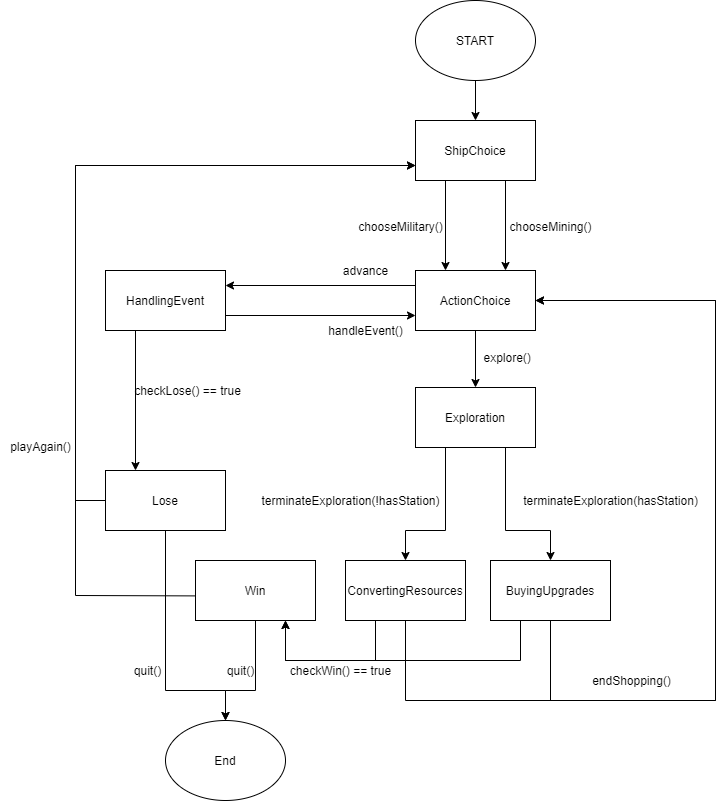
\includegraphics[scale=0.5]{StateDiagram.png}
\end{figure}

\newpage
\section{Classes}
My project is structured in the following way:
\begin{figure}[H]
	\caption{Package diagram}
	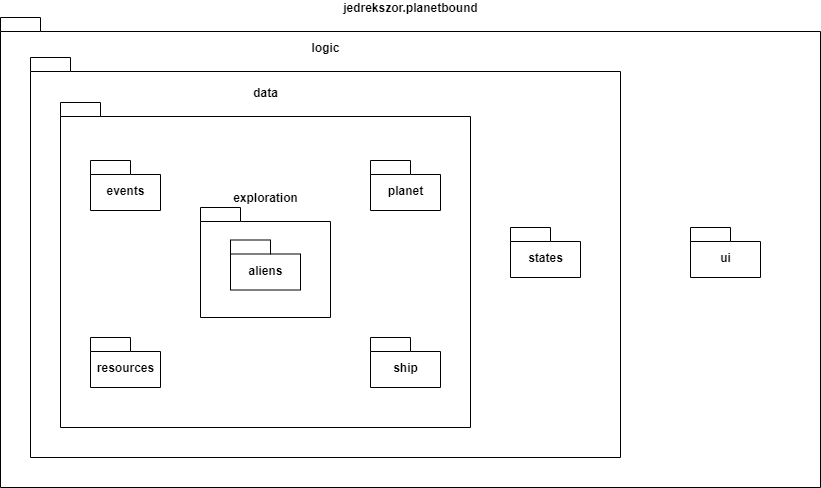
\includegraphics[scale=0.5]{PackageDiagram.png}
\end{figure}
The "ui" package contains controller classes responsible for controlling the widgets appearing on the screen. "Logic" package is responsible for the entire logic of the application. It contains classes performing all the actions as well as classes working as data structures. In that package there is also class Singleton which works as the main controller of the game containing all of the major objects and being able to be accessed from anywhere. The "states" package contains the abstract class State and classes representing all of the states, which inherit from the State class. "Data" contains classes working mostly as data structures and representing ship, alien, etc. Package "events" contains abstract class Event, descendant classes representing every event and the EventFactory class with static method for returning random event. "Planet" has very similar structure but contains also a Station class which can be an attribute of Planet if it has a space station orbiting around it. The "resources" package contains interface Resource, classes representing different resources, artefact and the ResourceFactory. I used an interface here and abstract classes in previous cases because I did not need the Resource class itself to have any methods, as I did with Planet, Event and Alien. Package "ship" contains an abstract class Ship and inheriting classes MiningShip and MilitaryShip. The "exploration" package contains all of the logic necessary for managing the part of the game happening on the surface of the planet. It contains an abstract class SurfaceWalker which is a base for both Drone and Alien. It also contains class Surface, which is the main controller of the logic on the planet's surface and class Coordinates, which represents the position of SurfaceWalker. Package "aliens" is very similar to the "planet", "events" and "resources". It contains an abstract class Alien, classes representing different Aliens and an AlienFactory.

\section{Relationships between classes}
\begin{figure}[H]
	\caption{Class relationship diagram without methods and attributes for better readability}
	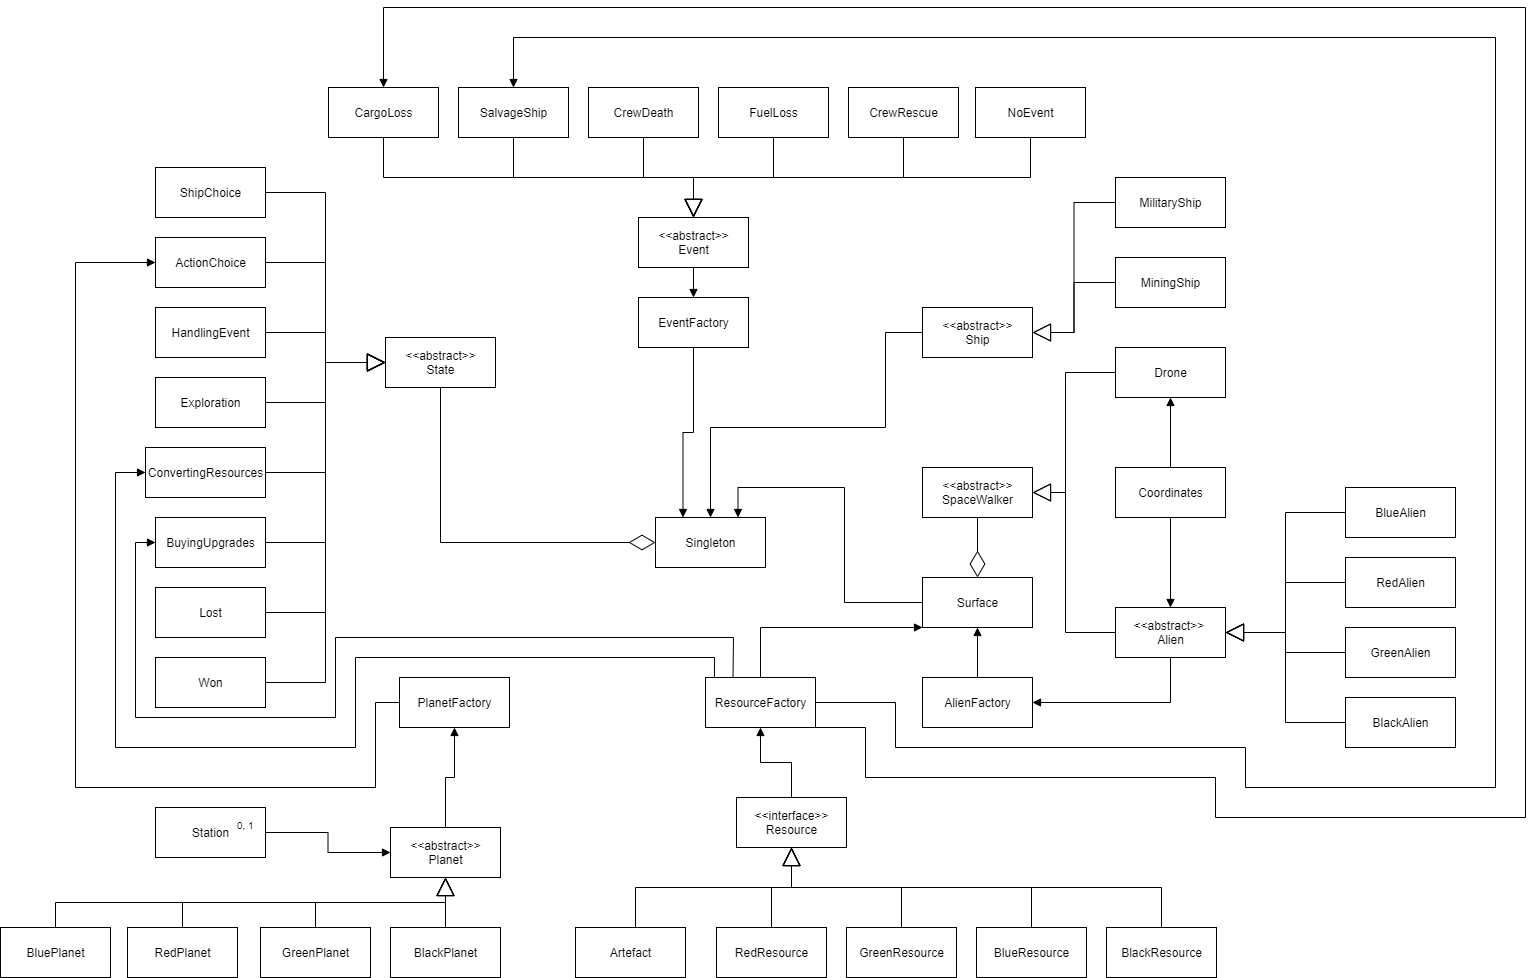
\includegraphics[scale=0.25]{ClassRelationship.png}
\end{figure}

\section{Status of implementation}
\begin{table}[H]
%	\begin{center}
		\begin{tabularx}{\linewidth}{|c|X|}
			\hline
			\textit{\textbf{Feature}} & \textit{\textbf{Status of implementation}}\\
			\hline
			Ship choice & Fully implemented\\
			\hline
			Proceeding to the next planet & Fully implemented\\
			\hline
			Drawing and resolving event & Fully implemented\\
			\hline
			Possibility to travel through a wormhole & Implemented, not yet tested\\
			\hline
			Possibility to land on the planet & Fully implemented\\
			\hline
			Movement on the surface of the planet & Fully implemented\\
			\hline
			Drawing and spawning aliens & Fully implemented\\
			\hline
			Aliens moving towards drone & Fully implemented\\
			\hline
			Fighting with aliens & Fully implemented\\
			\hline
			Buying resources & Fully implemented\\
			\hline
			Upgrading systems on station & Fully implemented\\
			\hline
			Win and lose conditions & Implemented, not yet tested\\
			\hline
			Possibility to play again & Implemented, not yet tested\\
			\hline
			Basic GUI & Almost fully implemented, lack of win and lose screens\\
			\hline
			Log system & Not yet implemented\\
			\hline
			\end{tabularx}
%	\end{center}
\end{table}


\end{document}